\documentclass[fontsize=12pt, paper=a4, headinclude, twoside=false, parskip=half+, pagesize=auto, numbers=noenddot, open=right, toc=listof, toc=bibliography]{scrreprt}
\usepackage[left=3cm, bottom=3cm, top=3cm]{geometry} % wenn es nicht anders geht sonst typearea (unten)
\usepackage{multirow} % Tabellen-Zellen über mehrere Zeilen
\usepackage{multicol} % mehre Spalten auf eine Seite
\usepackage{tabularx} % Für Tabellen mit vorgegeben Größen
\usepackage[automark]{scrpage2} % Kopf- und Fußzeilen
\usepackage[T1]{fontenc} % Ligaturen, richtige Umlaute im PDF 
\usepackage[utf8]{inputenc}% UTF8-Kodierung für Umlaute usw
\usepackage{bibgerm} % Bibliographie Umlaute in BibTeX
\usepackage{mathtools}

 
 \newcommand{\ourtitlepage}{
 %++++++++++++++++++++++++++++++++++++++++++++++++++++++++++++++++++
% Titelseite
%\clearscrheadings\clearscrplain
\begin{center}
{\large Universität Leipzig}\\
{\large Fakultät für Mathematik und Informatik}\\
{\large Institut für Informatik}\\
{\large Abteilung Automatische Sprachverarbeitung}\\
\vspace{5cm}
\begin{Large}
\textbf{Wortschatz Zeitgeist}\\
\vspace{5mm}
Seminararbeit\\
\vspace{5mm}
\end{Large}
\vspace{9cm}
\begin{tabular}{ r l }
{\bf Autoren:} 	& Döring, Thomas\\
			& Kießling, Max\\
			& Otto, Wolfgang (2885214)\\
{\bf Modul:} & Anwendungen Linguistische Informatik (10-202-2307)\\
{\bf Abgabe:} & {\today}. (Sommersemester 2015)\\
{\bf Betreuer:} & Maciej Janicki\\
{\bf Seminarleiter:}&Prof. Dr. Uwe Quasthoff\\ 
\end{tabular}\\
\end{center}
\clearpage

}


\begin{document}
\ourtitlepage 
\tableofcontents
\pagenumbering{roman} % Inhaltsverzeichnis roemisch 
\clearpage
\pagenumbering{arabic} % ab jetzt die normale arabische Nummerierung



% EINLEITUNG ###################################################################################
\chapter{Einleitung}

%##########################################
\section{Aufgabenstellung}
Das Portal  \emph{Wörter des Tages} (\url{http://wortschatz.uni-leipzig.de/wort-des-tages}) stellt eine Übersicht von Wörtern, die an einem ausgewählten Tag besonders relevant erschienen dar. Die Wörter sind in neun Kategorien eingeordnet. Nach der Beschreibung auf der Website werden die Wörter ermittelt in dem die tagesaktuelle Häufigkeit eines Wortes mit seiner durchschnittlichen Häufigkeit über längere Zeit hinweg gemessen wird.\\
Die Aufgabe dieser Arbeit ist es verschiedene Möglichkeiten der Bestimmung von Wörtern, die an einem gewählten Tag von besonderer Relevanz sind zu beschreiben, zu vergleichen und zu evaluieren. 
Die Datengrundlage zur Erstellung der Wörter des Tages ist ein Corpus, das durch tägliches crawlen von Newsseiten generiert wird. Die Quellen der Newseiten sind eine definierte Menge an für relevant erachtete Seiten mit Nachrichten wie zum Beispiel \emph{Spiegel.de}.\\
Bei allen Ansätzen, die auf das Vorkommen in einem Referenzzeitraum rekurrieren besteht das Korpus aus allen gecrawlten Newsseiten des voragngegangenen Jahres (2014).
Als Zusatzaufgabe soll ein musterbasiertes Verfahren in SQL entworfen werden, das es ermöglicht aufgrund eines gewählten Verfahrens falsch identifizierte Wörter zu filtern. Ein Beispiel hierfür sind Datumsangaben, die als relevant erscheinen, da sie Tagesaktuell oft auftauchen, aber im Vergleichszeitraum selten.

%##########################################
\section{Vergleichbare Ansätze}
Das Problem der Trenderkennung ist ein vielfältiges Problem mit einer großen Bandbreite an Anwendungsgebieten. Eine der vielleicht populärsten Anwendungen ist die Erkennung von Trendbegriffen bei Twitter, einem Microbloging-Dienst mehreren hundert Millionen Nutzern und 500 Mio Tweets täglich. Aufgrund dieser immensen Vielfalt an Nutzern und Nachrichten ist es möglich, dass hochaktuelle Nachrichten und Neuigkeiten rasend schnell global verbreitet werden können. Mithilfe von Trendanalyse ist es möglich globale aber auch lokale Entwicklungen zeitig zu erfassen und zu analysieren.
Einen ähnlichen Ansatz verfolgt das Google Projekt \emph{Google Trends}. Hier werden die Suchenanfragen der weltweit größten Websuchmaschine ausgewertet, wodurch die zeitabhängige Auswertung einzelner Suchbegriffe möglich wird. \\
Aber auch bei kleinerer Datenmengen ist das Erkennen von Trends bzw. Anomalien nützlich. Angewand auf Logdateien ist es so zum Beispiel möglich Angriffe auf ein Computersystem zu erkennen. \cite{Zwietasch14}


% HAUPTTEIL THEORIE ##########################################################################
\chapter{Methoden zum Finden tagesaktueller Wörter}
Im folgenden Abschnitt werden vier Methoden vorgestellt, die f\"uer jedes Wort eines Tageskorpus eine Ma\ss zahl bestimmen, die die Relevanz des Wortes an diesem Tag ausdr\"ucken soll.

%##########################################
\section{Maße zur Trend-Detection}

%#####################

\section{Relatives Vorkommen (Referenz)}
Ein einfacher Ansatz, der als Referenz zum Finden relevanter Wörter eines Tages dient ist der, das Auftreten jedes Tokens im Tageskorpus mit dem Auftreten im Referenzkorpus ins Verhältnis zu setzen.\\
Hierbei werden um eine Vergleichbarkeit zwischen verschiednen Tagen zu gewährleisten die Frequenzen der Wörter über die Anzahl aller Tokens im Tages bzw. Referenzkorpus normiert.\\

	\emph{Formel: } 
	\begin{equation}
	sig_{freqratio}(w) = \frac{\frac{k_{day}}{n_{day}}}{\frac{k_{2014}}{n_{2014}}}
	\end{equation}
	$k_{day}$: Frequenz des Tokens an einem Tag\\
	$n_{day}$: Summe der Frequenzen aller Tokens eines Tages\\
	$k_{2014}$: Frequenz des Tokens im Referenz Zeitrahmen (2014)\\
	$n_{day}$: Summe der Frequenzen aller Tokens im Referenzzeitraum (2014)\\
	

In Abbildung~\ref{pic.rel_freq} stellt die schwarze Gerade dar, wie sich der Wert der relativen Frequenz verhält, wenn die Anzahl des Auftretens eines Tokens variiert. Die senkrechte roten Linien markiert die Anzahl der Tokens, bei denen das relative Auftreten dem relativen Auftreten im Referenzkorpus entspricht. Der Wert der relativen Frequenz steigt also linear bei der Steigerung der Anzahl der Tokens eines Wortes.Dies führt zu der Problematik der Überschätzung von niederfrequenten Wörter im Referenzkorpus selbst bei relativ seltenem Auftreten im Tageskorpus. Bei niederfrequenten Wörtern ist der Anstieg der Gerade sehr viel steiler.\\
Um diesem Problem gerecht zu werden hilft es ein Maß für die Relevanz eines Wortes finden, welches ein geringe Überschreitung des relativen Anteils im Referenzkorpus weniger goutiert als eine höhere. Der Ansatz des Poisson Maß es (\ref{subsec.poisson}) versucht dem gerecht zu werden.\\
\begin{figure}[h!]
    \centering
    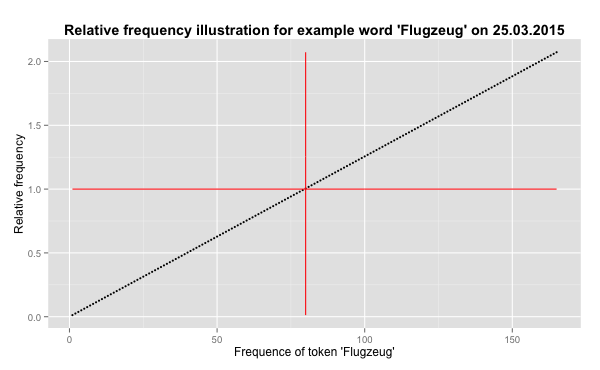
\includegraphics[width=1\textwidth]{pictures/relfreqFlugzeug.png}
    \caption{Illustration der relativen Frequenz des Tokens \enquote{Flugzeug} am 25.03.2015}\label{pic.rel_freq}
\end{figure}



\section{Poisson-Maß}\label{subsec.poisson}
Die Idee dieses Ansatzes ist es ein Maß zu nutzen, das die Wahrscheinlich Ausdrückt die gemessene Anzahl von Tokens eines Wortes an einem Tag zu beobachten. Auch hier wird zur Erstellung des Maßes  das Referenz

korpus des letzten Jahres genutzt. Die Annahme dieses Ansatzes ist nun, dass dieser Wahrscheinlichkeit die Poisson-Verteilung zugrundeliegt.\\
Die Formel~\ref{equ.poisson} ist die Poisson-Verteilung nach~\cite[S. 338 ff]{heyer06}.
	\begin{equation}\label{equ.poisson}
	P_\lambda(k) = \frac{\lambda^{k}}{k!}  \cdot e^{-\lambda}
	\end{equation}
	$\lambda$: Welche Frequenz wird erwartet \\
	(relativer Anteil im Referenzkorpus $\cdot$ Umfang des Tageskorpus)\\
	$k$: tatsächliches Auftreten von einem Wort k\\
	$P_\lambda(k)$: Erwartete Wahrscheinlichkeit meine Beobachtung k


In Abbildung~\ref{pic.poisson_algemein} ist exemplarisch die Wahrscheinlichkeit der Beobachtung der Token-Häufigkeit des Wortes Flugzeug abgebildet. Die Annahme besagt nun, dass je kleiner die Wahrscheinlichkeit
ist, desto relevanter erscheint ein Wort. \\

\begin{figure}[h!]
    \centering
    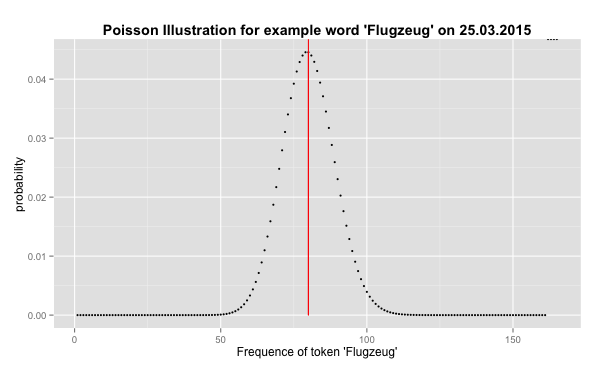
\includegraphics[width=1\textwidth]{pictures/poissonVerteilungFlugzeug.png}
    \caption{Illustration der Poissonverteilung des Token \enquote{Flugzeug} am 25.03.2015}\label{pic.poisson_algemein}
\end{figure}

An der Darstellung wird ein Nachteil dieser Methode deutlich. Nicht nur, wenn ein Token unerwartet oft beobachtet werden kann, auch wenn er seltener als erwartet beobachtet werden kann sinkt die Wahrscheinlichkeit nach diesem Modell beobachtet zu werden und es erscheint als relevantes Wort. Dieses Problem öst die im Folgenden beschriebene Transformation.\\

Ein weiteres Problem stellt der Rechenaufwand für diese Methode dar, da die Fakultät des tatsächlichen Auftretens $k$ eines Wortes berechnet werden muss. Die Herrleitung eines einfacher zu berechnenden 
equivalenten Maß es liefert~\cite[S. 338 ff]{heyer06}. Zu erwähnen ist, dass im Kontext dieser Herleitung wird das Maß allerdings nicht zur Bestimmung von in dieser Arbeit als relevant angesehenen Einzelwörtern genutzt. Sondern zur Bestimmung von signifikanten Kookurenzen. \\
Die Hergeleitete Formel~\ref{equ.poisson_mass} liefert drei Vorteile. Eine Berechnung der Fakultät ist nicht notwendig, die Anwendung des Logarithmus liefert ein positiven Wert für unwahrscheinliche Beobachtungen, wobei die differenzen gereade bei unwahrscheinlichen Beobachtungen stärker ins Gewicht fallen und yu letzt werden die Wahrschinlichkeiten für seltener als erwartete Tokenzahlen nicht berücksichtigt. 
 \begin{equation}\label{equ.poisson_mass}
		sig_{poisson}(w) = \frac{k(\log(k)-\log(n\cdot p) -1)}{\log(n)} 
 \end{equation}
k:= Anzahl der Token von w in Tagesbericht\\
n:= Anzahl der Tokens in Tagesbericht\\
p:= relativer Anteil eines Tokens am Jahreskorpus\\

Die Abbildung~\ref{pic.poisson_mass} illustriert die Entwicklung des Poissonmaß es bezogen auf die Variation des Vorkommens des Tokens Flugzeug. Hier wird sichtbar, dass die unterrepräsentetion keinen positiven Wert erzeugt und somit keinen Einfluss auf eine nach diesem Maß  geordnete Liste hat. In der Praxis sind genügend positive Werte dieses Maß es zu beobachten.\\
Die Formel~\ref{equ.poisson_mass} wurde im praktischen Teil dieser Arbeit genutzt.\\
 
% Hier Beispiel Flugzeug
\begin{figure}[h!]
    \centering
    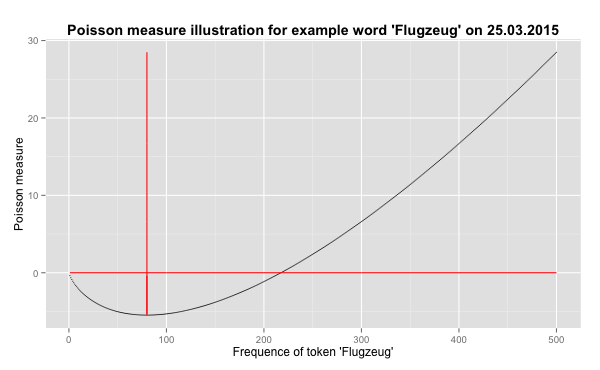
\includegraphics[width=1\textwidth]{pictures/poissonMeasureFlugzeug.png}
    \caption{Illustration des Poisson Maß es des Tokens \enquote{Flugzeug} am 25.03.2015}\label{pic.poisson_mass}
\end{figure}


\subsubsection{Bemerkungen zur Berechnung des Poisson-Maßes}
Die derzeitige Implementierung im Wortschatzporjekt der Universität Leipzig benutzt als Normierungsfaktor nicht die Anzahl aller Tokens im Tagesbericht. Auch zur Bestimmung des relativen Anteils eines Token am Jahreskorpus wird nicht die Anzahl der aller Tokens im Jahreskorpus, sondern die Anzahl der Sätze imJahreskorpus verwendet. Da bei der verwendeten Zahl von Sätzen das Verhältnis der Anzahl der Wörter zu der Anzahl der Sätze als konstant anzunehmen ist ($\approx 10$), scheint dies gerechtfertigt wie in~\ref{equ.word_sentence} formalisiert. 
\begin{equation}\label{equ.word_sentence}
\frac{|\text{Sätze}_{heute}|}{|\text{Sätze}_{jahr}|} \approx \frac{|Token_{heute}|}{|Token_{Jahr}|}
\end{equation}

Im Abschnitt~\ref{sec.quanitative_auswertung} wird diese Annahme durch einen Vergleich der sich ergebenden relevanten Wörter untersucht.

\section{Termfrequenz inverse Dokumentenfrequenz (tf-idf)}
Die Idee dieses Frequenzmaßes ist es, dass in der natürlichen Sprachverarbeitung breite Anwendung findende Maß TF/IDF für die Aufgabenstellung zu adaptieren. Dabei wird als Dokument das Korpus eines Tages im Referenzzeitraum betrachtet und für jedes Wort im Referenzzeitraum ein Wert bestimmt, der Angibt, an wie vielen Tagen das Wort im Jahr 2014 (Referenzzeitraum) aufgetreten ist. Verlgeiche dazu die Gleichung~\ref{equ.tfidf}.\\
\begin{equation}\label{equ.tfidf}
sig_{tf idf}(w) = \frac{k}{\max(K)} \cdot \log ( \frac{365}{|documentdays(w)|})
\end{equation}
$k$: Frequenz eines Tokens an einem Tag\\
$K$: Alle Frequenzen an einem Tag\\
Als Modifikation wird hier das gängige Verfahren der Logarithmisierung der inversen Dokumentfrequenz angewendet. Des weiteren wird, um eine Vergleichbarkeit über verschiedene Tage hinweg herrstellen zu könnnen, eine Relativierung der Frequenz auf Frequenz des häufigsten Tokens am Tag durchgeführt. Die graue Linie repräsentiert den idf-Wert, der zu der Entsprechung der relativen Tagesfrequenz führt, denn der Logarithmus von 2,7 ist ungefähr 1. Das entspricht dem Auftreten in ca. 8 Tagen des Referenzjahres.\\
% Hier Beispiel Flugzeug
\begin{figure}[h!]
    \centering
    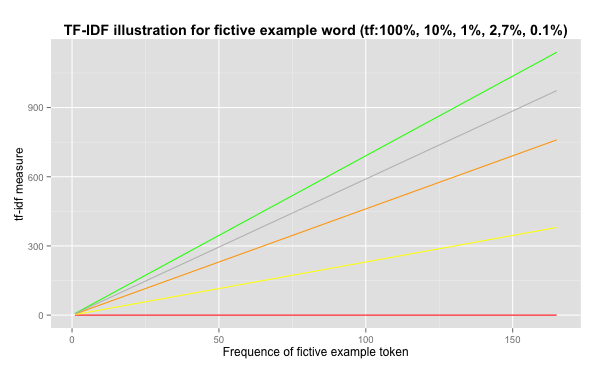
\includegraphics[width=1\textwidth]{pictures/tfidfIllustration.png}
    \caption{Illustration des TF/IDF Maßes anhand eines fiktiven Beispielworts}\label{pic.tfid_mass}
\end{figure}
Die Abbildung~\ref{pic.tfid_mass} verdeutlicht zwei Auswirkungen auf das Finden von relevanten Wörtern für die Aufgabenstellung. Zum einen ist das Grundlegende Problem, welches uns bei dem Maß des relativen Auftretens begegnete, dass niederfrequente Wörter überschätzt werden wieder vorhande, da mit steigender Frequenz die Maßzahl linear wächst. Allerdings wertet die inverse Dokumentenfrequenz häufige Wörter, wie Stoppwörter ab, was hilfreicht erscheint, da diese nicht als interessant zu bewerten sind.
Die rote Linie repräsentiert das Auftreten eines Worten an alle Tagen des Referenzkorpus. Die anderen Geraden bilden eine repräsentative Auswahl an weiteren Anteilen des Wortes an Tagen im Referenzjahr.\\

\section{Termfrequenz inverse Dokumentenfrequenz inverse Quellenfrequenz (tf-idf-isf)}
\emph{Idee: } Wörter sind dann interessant, wenn sie an einem Tag in möglichst vielen verschiedenen Quellen gennant werden.\\
Als Quelle definieren wir die Serveradresse einer Quelle. Diese wird mittels eines regulären Ausdrucks aus den zugeordneten Quellen in der MySQL-Datenbank ermittelt. Als Gesamtzahl der Quellen verwenden wir alle an einem Tag den Wörtern zugeordnete Quellen.\\
Das entstandene Signifikanzmaß wird in Gleichung~\ref{equ.tfidfsf} definiert.
\begin{equation}\label{equ.tfidfsf}
sig_{tf idf isf}(w) = sig_{tf idf}(w) \cdot \log ( \frac{Q_d}{q_d(w)})
\end{equation}
Analog zur inversen Dokumentenfrequenz wird also das tf-idf-Signifikanzmaß mit dem Logarithmus der inversen relativen Anzahl der Quellenfrequenz multipliziert. $Q_d$ ist die Anzahl aller erwähnten Quellen an einem Tag $d$ und $q_d()$ bildet ein Wort auf die Anzahl der Quellen ab, in denen das Wort an Tag $d$  erwähnt wird. 


%#####################
\subsection{Z-Score}
Benattar et al. beschreiben in \cite{benattar2011trend} einen Ansatz zur Trend-Erkennung basierend auf dem Z-Score. Dabei beziehen Sie neben der relativen Worthäufigkeit noch die Anzahl der Tage ein an denen ein Wort mindestens einmal auftritt, um so das 0-Frequenz-Problem zu umgehen.

\subsubsection{Berechnung}
\begin{itemize}
	\item{Wortfrequenz}\\
		$f(w)_d :=$ Anzahl der Vorkommen von Wort $w$ an Datum $d$
	\item{relative Worthäufigkeit}\\
		Die relative Worthäufigkeit $p(w)_d$ berechnet sich durch: \\
		$t_d :=$ Anzahl verschiedener Worte an Datum $d$
		$$ p(w)_d = \frac{f(w)_d}{t_d} \\ $$
	\item{Erwartungswert}\\
		Der Erwartungswert $\bar{w}$ berechnet sich durch: \\
		$N:=$ Anzahl der Tage in der betrachteten Zeitspanne
		$$\bar{w}=\frac{1}{N} \sum p(w)_d$$
	\item{Standartabweichung}\\
		Die Standartabweichung $\sigma_w$ berechnet sich durch:
		$$\sigma_w = \sqrt{\frac{1}{N} \sum (p(w)_d - \bar{w}^2}$$
	\item{ZScore}\\
		Der Zscore $Z(w)_d$ misst die Abweichung der relativen Worthäufigkeit vom Erwartungswert in Vielfachen der Standartabweichung.
		$$Z(w)_d= \frac{p(w)_d - \bar{w}}{\sigma_w}$$		
	\item{Auftrittshäufigkeit}\\
		Die Auftrittshäufigkeit $Po(w)$ gibt an wie vielen Tagen innerhalb des betrachteten Zeitraums das Wort mindestens einmal auftritt:\\
		$nbD(w) :=$ Anzahl der Tage an denen $w$ vorkommt//
		$c_d:=$ Anzahl der Tage innerhalb des betrachteten Zeitraums
		$$Po(w)=\frac{nbD(w}{c_d}$$
	\item{Schwellwerte}
		Zur besseren Unterscheidung echter Trends von statistischen Anomalien schlagen Benattar et. al. vor die Worte anhand ihrer Auftrittshäufigkeit zu clustern. Den Clustern werden dabei Z-Score-Schwellwerte zugeordnet. Überschreitet der Z-Score eines Wortes den Schwellwert seines Clusters wird dieses Wort als signifikant und somit als Trend eingestuft. Cluster mit niedriger Auftrittshäufigkeit erhalten dabei höhere Schwellwerte. Je häufiger ein Wort auftritt desto niedriger wird der Schwellwert. 
		
		
\end{itemize}

\subsubsection{Vorgehen}
\begin{enumerate}
	\item Für jedes Wort in $w$ in $d$ berechne $Z(w)$
	\item 
\end{enumerate}


%#####################
\subsection{Weitere Maße}
Einbeziehung der Anzahl von Quelle

%##########################################
\section{Zeitreihenanalysen}

%##########################################
\section{Cleaning}
Es sollen Datumsangaben und evtl. neu auftauchende strukturelle Angaben ausgefiltert werden.\\
Ansatz: Regelbasiert.\\
Gibt es Maße, die solche Angaben strukturell ausschließen?



%HAUPTTEIL IMPLEMENTIERUNG ##################################################################
\chapter{Implementierungen in SQL und R}



% AUSWERTUNG #################################################################################
\chapter{Ein empirischer Vergleich}
 
Kriterien: Anteil niederfrequenter Wörter in der Top-Liste\\
\section{Einleitung}
Die Messung der G\"ute der Ergebnisse stellt eine Herausforderung dar, da es keine geeignete Referenz, beispielswiese in Form eines Goldstandards der wichtigsten Worte eines Tages gibt. Um die G\'ute trotzdem einsch\"atzen zu k\"onnen bieten sich zwei herangehensweisen an. Zum einen die eigenst\"andige manuelle Pr\"ufung der Ergebnisse unter selbst formulierten Kriterien, zum anderen der quantitative Vergleich mittels eines geeigneten Abstandsma\ss es. Letzterer Ansatz bietet aber nur die M\"oglichkeit eines Verlgeiches der \"Ahnlichkeiten der Ergebnisse und hilft abzusch\"atzen wie sich die Ergebnisse gegeneinander verhalten. \"Uber die G\"ute gibt diese Methode keine Auskunft. Allerdings lassen sich Ausrei\ss er gut erkennen und der Pr\"amisse, dass gleiche Ergebnisse, die aus verschiedenen M\"ass ungen stammen eine h\"ohere Wahrscheinlichkeit besitzen gute Ergebnisse zu sein l\"asst sich auch die Qualit\"at beurteilen.
\section{Qualitativer Vergleich}
Um sich einen Eindruck der Ergebnisse anhand der resultierenden soriterten Wortlisten zu verschaffen wurden die Listen ausgew\"ahlter Tage verglichen. Da die Untersuchenden keine ausgewiesene Expertiese ausweist, die wichtigsten W\"orter eines t\"aglichen Nachrichtenstroms zu indentifizieren, die \"uber der eines Zeitungslesers liegt kann die Analyse nicht in die Tiefe gehen. Aber durch die Wahl der Tage l\"asst sich das \"Uberblicken der Ergebnisse vereinfachen. Deshalb w\"ahlten wir den 1.1.2015. \\
 Das funktiuoniert so noch nicht!!! Umschreiben ist nur blabla!!
\section{Quantitativer Vergleich - Average Overlap als Vergleichma\ss}
\subsection{Einf\"uhrung}
Der Vergleich zweier mit einer Rangfolge versehenen Listen ist ein bekanntes Problem. In unserem Fall handelt es sich um den spezialfall von Listen gleicher und fester L\"ange, aber einer potentiell unendlichen Zahl verschiedener W\"orter. Desweiteren sind die Listen nicht \emph{Conjoint}, was bedeutet, dass nicht nur gemeinsame W\"orter in den verschiedenen Listen auftauchen. In \cite{webber2010similarity} werden als Einleitung f\"ur ein Ma\ss, dass in der Lage ist auch unendliche Listen und Listen verschiedener L\"ange vergleichen zu k\"onnen geeignete Verfahren vorgestellt um solche Listen zu vergleichen. Das gew\"ahlte Verfahren \emph{Average Overlap} wird von den Autoren als \emph{top-k ranking} identifiziert. Also ein Ranking bis zu einer definierten Tiefe von k.\\
Der Vorteil des genutzten Verfahrens f\"ur unseren Anwendungsfall ist, dass der Rang der W\"orter einen Einfluss auf das Ma\ss haben. \"Ahnlichkeiten an der Spitze der Liste werden st\"arker gewichtet.\\
Das Verfahren ist ein Mengenbasierter Ansatz. Listen sind sich dann \"ahnlich, wenn sie die relative Anzahl gemeinsamer W\"orter hoch ist. Um nun aufsteigende Gewichtungen zu erhalten wird nun nicht nur die gesamte \"Uberlappung zweier Listen gemessen, sondern die Listen in K Listen unterteilt, wobei K die L\"ange der Listen ist und jede einzelne Liste jeweils alle Elemente bis zu dem Rang des Laufindexes k von 1 bis K enth\"alt. Also eine Liste der Form: [[ Wort 1],[Wort 1, Wort 2], ...]. Nun wird bei den einzelnen Listen gleicher L\"ange die relative \"Uberlappung gemessen. Um nun das Verlgleichsma\ss  zu erhalten wird der Durchschnitt aller errechneten Werte gemessen.  Formalisiert ergibt dies:
\begin{equation}
AO(S,T) = \frac{\sum_{k=1}^K\frac{| M(S_k) \cap M(T_k)|}{k}}{K}
\end{equation}
Wobei $S$ und $T$ zwei Listen sind, der tiefgestellte Index $k$ die Teilliste bis zum Rang $k$ angibt und $K$ die L\"ange der beiden Listen definiert. $M$ ist hierbei die Abbildung einer Liste auf die Menge der enthaltenen Elemente.\\
%Beispiel:\\
\subsection{Ergebnisse}
Hier die Ergebnisse f\"ur den 1.5.2015 mit der Listenl\"ange $K=1000$
\begin{table}[ht]
\centering
\begin{tabular}{rllr}
  \hline
 & List & List\_to\_compare & average\_overlap \\ 
  \hline
1 & tf\_idf & poisson & 0.66 \\ 
  2 & tf\_idf & z-score & 0.18 \\ 
  3 & tf\_idf & freqratio & 0.31 \\ 
  4 & tf\_idf & freqratio\_old & 0.31 \\ 
  5 & tf\_idf & poisson\_old & 0.66 \\ 
  6 & poisson & z-score & 0.15 \\ 
  7 & poisson & freqratio & 0.16 \\ 
  8 & poisson & freqratio\_old & 0.16 \\ 
  9 & poisson & poisson\_old & 1.00 \\ 
  10 & z-score & freqratio & 0.16 \\ 
  11 & z-score & freqratio\_old & 0.16 \\ 
  12 & z-score & poisson\_old & 0.15 \\ 
  13 & freqratio & freqratio\_old & 1.00 \\ 
  14 & freqratio & poisson\_old & 0.16 \\ 
  15 & freqratio\_old & poisson\_old & 0.16 \\ 
   \hline
\end{tabular}
\caption{Avarage Overlap Comparison} 
\label{AvarageOverlapComparison}
\end{table}\begin{figure}[htbp] 
  \centering
     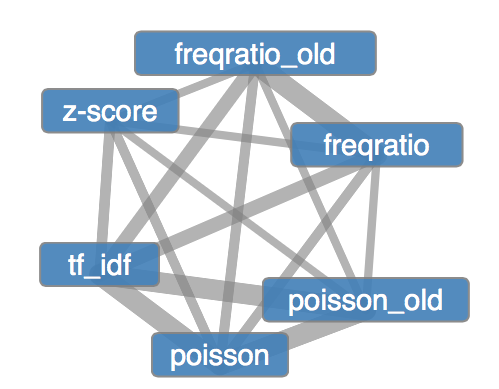
\includegraphics[width=0.7\textwidth]{pictures/comparison.png}
  \caption{Graph of Average Overlap}
  \label{fig:comparisonGraph}
\end{figure}




% SCHLUSS #####################################################################################
\chapter{Bewertung und Zusammenfassung}



% LITERATUR ####################################################################################
\nocite{*}%alle nicht aufgeführte Literatur auch auffuehren
\bibliographystyle{plaindin} %alphadin_martin
\bibliography{wortschatzZeitgeistLit} 

\end{document}